\vspace{-1mm}


\section{HVI vs. LLMs size for different LLMs: An insight from 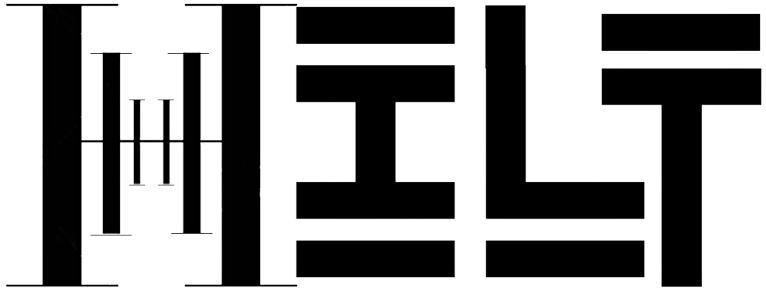
\includegraphics[width=1cm]{img/hilt.png}}

There is a general observation that LLMs may exhibit a higher tendency towards generating hallucinations or producing outputs that deviate from factual or coherent information. However, it is important to note that the relationship between LLM size and hallucination is not necessarily a direct correlation, but rather a consideration based on certain factors such as (a) training data quality, (b) lack of explicit training on facts, and (c) overconfi-

\begin{figure}[!]
    \centering
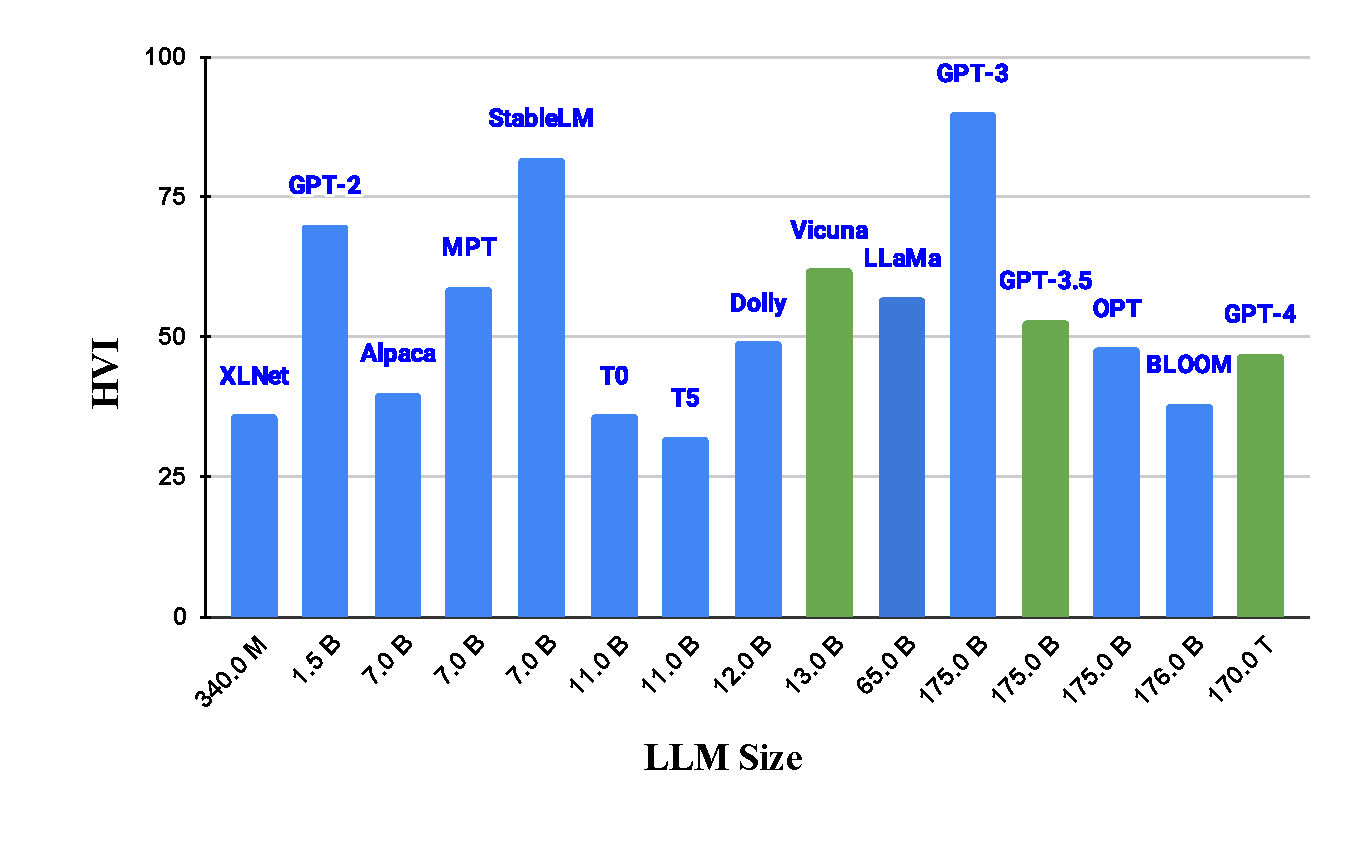
\includegraphics[width=0.99\columnwidth]{img/chart1.pdf}
    \caption{\emph{HVI} vs. \emph{LLM size} for different LLMs. \textcolor{ForestGreen}{Green} indicates LLMs using RLHF.}
    \vspace{-4mm}
    \label{fig:llm-size}
\end{figure}
\noindent 
dence in generated responses. A noteworthy pattern that emerges is that LLMs without RLHF (Reinforcement Learning from Human Feedback) \cite{DBLP:journals/corr/abs-1909-08593} tend to exhibit a higher tendency for hallucination. Although we did not extensively evaluate this phenomenon, we have a keen interest in investigating it further in the near future. While we tried to examine the effect of size on HVI, it looks like there are several other factors contributing to HVI behavior as evident in \cref{fig:llm-size}.



\vspace{-1mm}
\section{Hallucination Mitigation Strategies}
\label{sec:mitigation}
\vspace{-1mm}
%\textbf{brief on proposed mitigation strategies:}
Thus far, two classes of approaches have been proposed to address the issue of hallucination: (i) preventing LLMs from hallucinating, which involves implementing strategies during the training and/or generation processes; (ii) mitigating hallucination after generation. 
% The latter has garnered significant attention recently. 
\cite{manakul2023selfcheckgpt} introduced another taxonomy of classification, categorizing methods into \emph{black-box} and \emph{gray-box}. 
Factuality checks during and/or after generation without relying on external resources are known as black-box methods, while those using external resources are referred to as gray-box methods.
% The terms \emph{black-box} and \emph{gray-box} were introduced by \cite{manakul2023selfcheckgpt}. Gray-box methods can be compared to fact-checking techniques used for verifying the authenticity of fake news \cite{fake_news_verification_reference}. On the other hand, incorporating fact-checking during the generation process represents a novel paradigm that warrants further exploration. Black-box methods, on the other hand, require access to token-level probabilities, which are often available only through paid APIs for many contemporary Language Models (LLMs). This presents a more complex yet demanding paradigm, as emphasized by \cite{manakul2023selfcheckgpt}.}
% \textbf{A brief discussion on other available mitigation techniques:} 
%\vspace{-1mm}

Other hallucination mitigation techniques involve reranking the generated sample responses \cite{dale2022detecting} and improving beam search \cite{sridhar2022improved}. Some recent mitigation techniques \cite{li2023halueval,mündler2023selfcontradictory,pfeiffer2023mmt5,chen2023purr,zhang2023mitigating,zhang2023language,ladhak-etal-2023-pre,manakul2023selfcheckgpt,agrawal2023language} show initial attempts at reducing hallucination. %\textcolor{red}{Need to rephrase this last statement.} 

Although the complete elimination of hallucination is a complex challenge, this paper explores two plausible directions for mitigation: (i) automatic and (ii) human-in-the-loop. The former is a black-box method where we identify high-entropy words in a given hallucinated text (generated by a high-HVI LLM) and replace them with predictions from another LLM (lower-HVI). The latter is a gray-box method that involves sentence-level fact-checking using textual entailment techniques. This method aims to identify sentences that are deemed susceptible, urging them for human review.


\vspace{-1mm}
%GPT-3
\begin{table}[!htp]
\centering
\scriptsize
\resizebox{\columnwidth}{!}{%
\begin{tabular}{lrrrrr}\toprule
\textbf{} &\textbf{\texttt{ALBERT}} &\textbf{\texttt{BERT}} &\textbf{\texttt{DISTIL-ROBERTA}} &\textbf{\texttt{XLM-ROBERTA}} \\\midrule
\textbf{\texttt{ALBERT}} &\cellcolor[HTML]{93c47d}6.72 &\cellcolor[HTML]{f6b26b}3.26 &\cellcolor[HTML]{76a5af}\textbf{10.66} &\cellcolor[HTML]{93c47d}6.40 \\
\textbf{\texttt{BERT}} &\cellcolor[HTML]{ffd966}4.70 &\cellcolor[HTML]{93c47d}7.56 &\cellcolor[HTML]{93c47d}7.98 &\cellcolor[HTML]{93c47d}7.22 \\
\textbf{\texttt{DISTIL-ROBERTA}} &\cellcolor[HTML]{f6b26b}2.02 &\cellcolor[HTML]{93c47d}7.31 &\cellcolor[HTML]{ffd966}4.55 &\cellcolor[HTML]{76a5af}9.95 \\
\textbf{\texttt{XLM-ROBERTA}} &\cellcolor[HTML]{f6b26b}2.26 &\cellcolor[HTML]{93c47d}6.28 &\cellcolor[HTML]{e06666}1.70 &\cellcolor[HTML]{ffd966}4.78 \\
\bottomrule
\end{tabular}%
}
\vspace{-1mm}
\caption{\textls[-5]{The row represents the LLM used for detecting high entropy words from GPT-3's output, while the column represents the LLM for replacing those words. \textbf{10.66} indicates the maximum drop in hallucination.}}
\label{tab:mitigation}
\end{table}
%\vspace{-4mm}

\vspace{-4.5mm}
\subsection{\textls[0]{High Entropy Word Spotting and Replacement (ENTROPY\textsubscript{BB}): A Black-box approach}}
\vspace{-1mm}
%\adt{To mitigate the occurrence of hallucination in generated text, one effective approach is to target and replace high-entropy points. High entropy points are segments of text where the LLM exhibits increased uncertainty and deviates from factual information. By identifying and replacing these points, we can effectively minimize the likelihood of hallucination or the generation of inaccurate content.}
%This approach contributes to the development of more trustworthy and contextually appropriate text generation systems, enabling their effective utilization in various applications. 

%\noindent
%\adt{\textbf{Detection and replacing high entropy points:} 
%\noindent
%\textbf{ENTROPY\textsubscript{BB} -High Entropy Word Spotting and Replacement:} 
While detecting high entropy words may seem to be technically feasible, there is an inherent challenge that many modern LLMs are not open-source (their APIs are subscription-based). The feasible solution we propose here is the utilization of open-source LLMs to identify high entropy words. A lower HVI-based LLM is then used to replace the detected words (see \cref{tab:hallucination_ex}). The outcomes of the detection and replacement strategies discussed earlier are presented in \cref{tab:mitigation} for GPT-3. 
% The results indicate that all the language models evaluated in this study exhibit similar performance in detection. However, when it comes to word replacement, BERT outperforms the other models and demonstrates the highest efficacy. 
The results indicate that \texttt{albert-large-v2} \cite{lan2020albert} performs exceptionally well in detecting high entropy words in GPT-3-generated content. On the other hand, \texttt{distilroberta-base} \cite{Sanh2019DistilBERTAD} demonstrates superior performance in replacing high entropy words, which in turn, manifests as a lower hallucination. A crucial aspect of our approach is treating consecutive high-entropy words as a single unit. In such cases, these words are masked together before replacement. This strategy proves to be effective, particularly for hallucinations related to Generated Golem or Acronym Ambiguity (cf. \cref{app:bb}).

\subsubsection{Lowering Concreteness of Language}
It is observed in \cite{varshney2023stitch} that higher uncertainty in the model's prediction (indicated by a low probability score) suggests a higher likelihood of the model hallucinating about that particular concept. In this context, we suggest that substituting high entropy points with less concrete words can help prevent hallucinations. 
%Consider the example (see \cref{tab:hallucination_ex}), where ``United States'' was replaced with ``government,'' the latter being a less concrete word. 
Concreteness \cite{paivio2013dual} measures how much a word embodies a tangible or perceivable concept. Concrete words are simpler to comprehend than abstract ones. The level of concreteness for each word is denoted on a 5-point scale, ranging from abstract to concrete. Concreteness ratings cover 39,954 entries, including 37,058 individual English words and 2,896 two-word expressions \cite{brysbaert2014concreteness}, being used here.


%old
\begin{comment}
%\vspace{-1mm}
\begin{table}[!h]
\centering
%\scriptsize
\vspace{-3mm}
\resizebox{\columnwidth}{!}{
\begin{tabular}{lccccccc}\toprule 
% \textbf{GPT-3.5} & & & & & \\\midrule 
& \textbf{BERT} & \textbf{RoBERTa} & \textbf{DeBERTa} & \textbf{T5} & \textbf{XLNet} & \textbf{ERNIE} \\\toprule
\textbf{LLaMA} &\cellcolor[HTML]{f6b26b}0.23 &\cellcolor[HTML]{76a5af}0.96 &\cellcolor[HTML]{f6b26b}0.29 &\cellcolor[HTML]{f6b26b}0.30 &\cellcolor[HTML]{f6b26b}0.40 &\cellcolor[HTML]{ffd966}0.60 \\
\textbf{GPT-2} &\cellcolor[HTML]{93c47d}0.80 &\cellcolor[HTML]{f6b26b}0.20 &\cellcolor[HTML]{76a5af}1.00 &\cellcolor[HTML]{f6b26b}0.40 &\cellcolor[HTML]{93c47d}0.75 &\cellcolor[HTML]{76a5af}0.99 \\
\textbf{Alpaca} &\cellcolor[HTML]{ffd966}0.60 &\cellcolor[HTML]{ffd966}0.59 &\cellcolor[HTML]{f6b26b}0.21 &\cellcolor[HTML]{e06666}0.11 &\cellcolor[HTML]{e06666}0.00 &\cellcolor[HTML]{76a5af}1.00 \\
\bottomrule
\end{tabular}%
}
\vspace{-1mm}
\caption{The row represents the LLM used for detecting high entropy words from GPT-3.5's output, while the column represents the LLM for replacing those words.}
\label{tab:mitigation}
\vspace{-2mm}
\end{table}
\vspace{-2mm}
\end{comment}




%A language model outputs a probability distribution over sequences of tokens. We find high entropy tokens with low probability. This can be achieved through methods such as measuring the entropy of the model's distribution over possible words or phrases at each point in the generated text. 
%In our research, we classify points with a probability lower than 40\% as high entropy points. These points exhibit a higher degree of uncertainty and lack clear consensus in the model's predictions. 
%The presence of high entropy points in text generation signifies unreliable model predictions that deviate from accurate and contextually appropriate information, leading to hallucinated text. Identifying and understanding these points is crucial for addressing hallucinations.


%\textbf{Replace high entropy points} From the available probability distribution for the LLMs, we substitute the token with a low probability for an LLM with a smaller LLM prediction of the same token. 

%Our research study focused on minimizing entropy and improving the quality of the generated text. We employed a masking-based approach, utilizing masking-based models to identify and replace low-probability points. By replacing these points, we successfully reduced the overall entropy of the generated text. Our findings highlight the significance of addressing low-probability points in text generation to enhance coherence and reliability. 

\vspace{-1mm}
\subsection{\textls[-20]{Factuality Check of Sentences (FACTUALITY\textsubscript{GB}): A Gray-box approach}}
% \vspace{-1mm}
%\noindent
%\textbf{FACTUALITY\textsubscript{GB} - Factuality Check of Sentences:} 
We use Google Search API \cite{googlesearchapi} to search for a given prompt, which has been utilized to generate the text and retrieve the top 20 documents. Then each sentence of AI-generated text has been validated either into \emph{support}, \emph{refute}, or \emph{not enough information} using RoBERTa Large \cite{liu2019roberta}, a SoTA textual entailment model trained on the SNLI \cite{bowman2015snli} (cf. \cref{app:gb}). Inevitably, sentences with higher scores in the \emph{refute} and \emph{not enough information} categories are flagged for additional human checking. Empirically, we observe an overall alert rate of 26\% on sentences generated by an LLM, implying 26\% of the text required rewriting in order to mitigate.


%from appendix

\subsubsection{FACTUALITY\textsubscript{GB}}
\label{app:gb}
Gray-box model \textbf{does} require output token-level probabilities \cite{manakul2023selfcheckgpt}. \cref{fig:fgb_illustration} shows \textbf{FACTUALITY\textsubscript{GB}}, representing AI-generated text (from our HILT benchmark) based on a given prompt. In this method, the prompt is sent to the Google Search API to obtain the top 20 relevant search results. Out of these 20 results, we evaluate a total of $n$ sentences for their relevance to the prompt using a similarity measure. The top 20 sentences most similar to the prompt are selected. For each of the $m$ sentences in the AI-generated text and the top 20 ranked sentences, we employ a textual entailment model to assess their trustworthiness individually. Based on their entailment scores, we categorize the AI-generated text into three groups: (i) \textit{support}, (ii) \textit{refute}, and (iii) \textit{not enough information}.


\begin{figure}[!ht]
    \centering
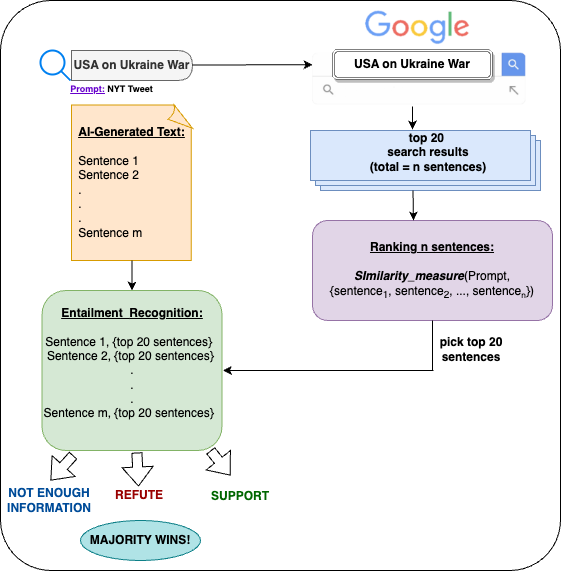
\includegraphics[width=0.99\columnwidth]{img/hilt_illustration.png}
    \caption{FACTUALITY\textsubscript{GB}: textual entailment on prompt and external documents.}
    \label{fig:fgb_illustration}
\end{figure}


\vspace{-2mm}
\textbf{Performance of ENTROPY\textsubscript{BB} vs. FACTUALITY\textsubscript{GB}:} \cref{fig:mitigation_all} offers a comparative analysis of the proposed approaches. While ENTROPY\textsubscript{BB} addresses simpler hallucinations such as Acronym Ambiguity and Numeric Nuisance, FACTUALITY\textsubscript{GB} handles more complex cases. It is clear that a balanced combination of black-box and gray-box approaches is the inevitable future avenue (cf. \cref{app:pp}).





%From these documents, we fetch top $k$ (based on an empirical threshold) sentences to classify into \emph{support}, \emph{refute}, or \emph{not enough information}. We calculate all three scores for a given sentence and choose the maximum likelihood. We employ RoBERTa Large \cite{liu2019roberta}, a SoTA model trained on the SNLI task for entailment. Upon obtaining sentence similarity scores, we rank them. Inevitably, sentences with higher scores in the \emph{refute} and \emph{not enough information} categories are flagged for additional human checking. Empirically, we observe an overall alert rate of 26\% on sentences generated by an LLM, implying that 26\% of the text required rewriting in order to alleviate hallucination.}

%Given a text snippet we break it down to sentences and search in Google using search API. Top 20 results are chosen to verify factual correction of the given sentence. At this step, we identify the examples which are entailed, and only those are chosen. For the entailment task, we have utilized RoBERTa Large \cite{liu2019roberta} -- a SoTA model trained on the SNLI task \cite{bowman2015large}. 


\begin{comment}
\begin{table*}[!ht]
\centering
\resizebox{0.7\textwidth}{!}{%
\begin{tabular}{ | p{0.07\textwidth} |
                   p{0.54\textwidth} | p{0.55\textwidth} |
                 }
\toprule
\textbf{Prompt} &
  Will the next great writer be a robot? &
  AI-generated text is impossible to detect! 
   \\ \hline
\rotatebox[origin=r]{90}{\parbox[c]{5cm}{\centering \textbf{AI-generated hallucinated text}}} &
    {I'm \colorbox{pink}{very skeptical} that the next ``great writer'' is going to be a robot, \colorbox{pink}{or} that they'll be \colorbox{pink}{much} more effective at \colorbox{pink}{expressing the} subtleties and depths of \colorbox{pink}{human} thought than a human is. However, what is \colorbox{pink}{most} interesting is the role that the \colorbox{pink}{Internet could} play in bringing these ''robot'' writers into the public eye. If I could (and I'm \colorbox{pink}{very} excited by this possibility), I would pay a \colorbox{pink}{small monthly} fee to \colorbox{pink}{read well-written}...} &
 { AI-generated text can be challenging to detect, especially with the advancements in natural language processing and machine learning. However, it is not accurate to say that AI-generated text is impossible to detect. There are various techniques and tools available that can help in identifying AI-generated content. Researchers and developers are actively working on improving detection methods to keep up with the evolving capabilities of AI models. While it may be difficult to distinguish between human-written and AI-generated text in some cases, ongoing efforts are being made to enhance detection and maintain transparency in communication.}
   \\ \hline
\rotatebox[origin=r]{90}{\parbox[c]{5cm}{\centering \textbf{De-hallucinated text by replacing high-entropy words}}} &
    {I'm \colorbox{green}{somewhat} skeptical that the next ``great writer'' is going to be a robot, \colorbox{green}{given} that they'll be \colorbox{green}{far} more effective at \colorbox{green}{grasping deeper} subtleties and depths of philosophical thought than a robot is. However, what is \colorbox{green}{particularly} interesting is the role that the Internet \colorbox{green}{may} play in bringing new great writers into the public eye. If I did (and I'm \colorbox{green}{extremely} excited by this possibility), I would pay a \colorbox{green}{hefty subscription} fee to \colorbox{green}{publish  something}...} & 
{AI-generated text can be challenging to detect, especially with the advancements in natural language processing and machine learning. However, it is not accurate to say that AI-generated text is impossible to detect. There are various techniques and tools available that can help in identifying AI-generated content. Researchers and developers are actively working on improving detection methods to keep up with the evolving capabilities of AI models. While it may be difficult to distinguish between human-written and AI-generated text in some cases, ongoing efforts are being made to enhance detection and maintain transparency in communication. }
   \\ \bottomrule
\end{tabular}
}
\caption{De-hallucination example}
\label{tab:my-table}
\end{table*}
\end{comment}

% \begin{figure*}
%   \begin{minipage}[t]{.65\linewidth}
%     \centering
%     % \includegraphics{example-image-duck}%
%     \begin{figure}
% [!htbp]
    \centering
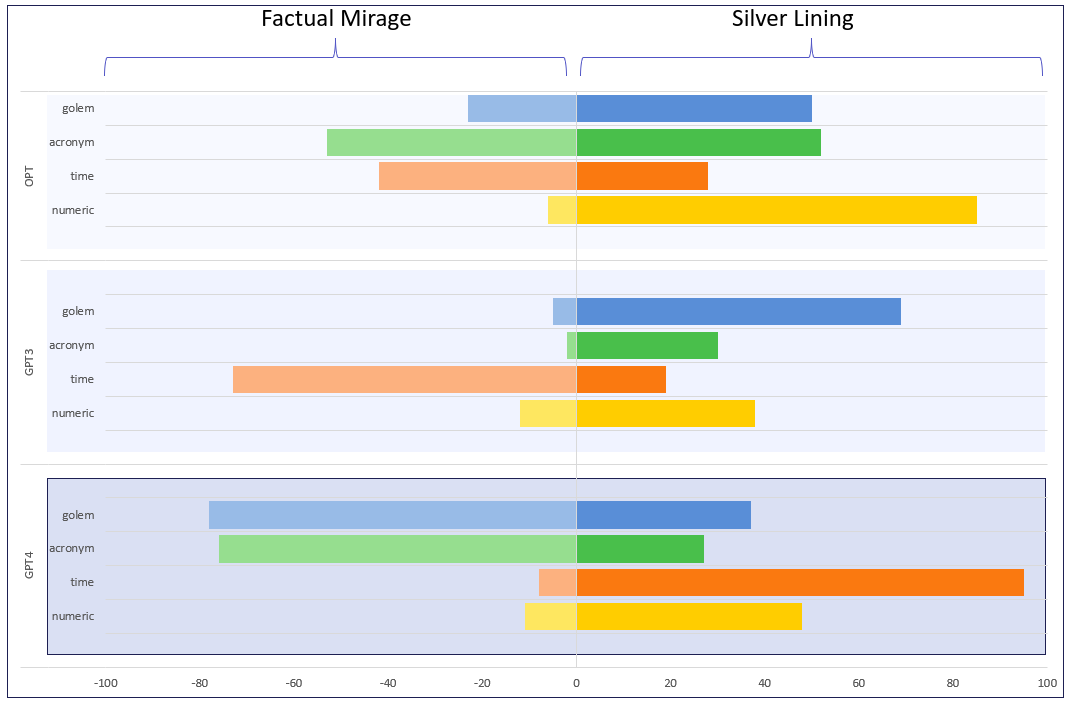
\includegraphics[width=\textwidth,height=9cm]{img/hvi.png}
    \caption{Hallucination Vulnerability Index \emph{(HVI)} for different hallucination categories for various LLMs \textcolor{red}{why does this figure have an arxiv link?}}
    \label{fig:hvi}
\end{figure}
%   \end{minipage}
%   % \hfill
%   \begin{minipage}[t]{.35\linewidth}
%     \centering
%     %\begin{table}[!ht]
%\tiny
%\centering
%\resizebox{0.32\textheight}{!}{%
\resizebox{0.9\columnwidth}{!}{%
\begin{tabular}{lll}
\toprule
\textbf{LLM} & \textbf{Size} & \textbf{HVI (0-100)}
\\ \midrule
\textbf{GPT-3}    &  175B       &   90 - 
\begin{tikzpicture}
\centering
\draw[red, very thick, fill=red] (0,0)  rectangle (5.62,.1);
\end{tikzpicture}
\\
\textbf{StableLM}    &  7B   &     82 - 
\begin{tikzpicture}
\centering
\draw[red, very thick, fill=red] (0,0)  rectangle (5.12,.1);
\end{tikzpicture}
\\
\textbf{GPT-2}    &   1.5B      &     70 - 
\begin{tikzpicture}
\centering
\draw[red, very thick, fill=red] (0,0)  rectangle (4.38,.1);
\end{tikzpicture}
\\
\textbf{Vicuna}     & 13B      &   62 - 
\begin{tikzpicture}
\centering
\draw[orange, very thick, fill=orange] (0,0)  rectangle (3.88,.1);
\end{tikzpicture}  
\\
\textbf{MPT}    &  7B    &     59 - 
\begin{tikzpicture}
\centering
\draw[orange, very thick, fill=orange] (0,0)  rectangle (3.69,.1);
\end{tikzpicture}   
\\
\textbf{LLaMA}    &  65B    &     57 - 
\begin{tikzpicture}
\centering
\draw[orange, very thick, fill=orange] (0,0)  rectangle (3.56,.1);
\end{tikzpicture}   
\\
\textbf{GPT-3.5}   &    175B      &     53 - 
\begin{tikzpicture}
\centering
\draw[orange, very thick, fill=orange] (0,0)  rectangle (3.31,.1);
\end{tikzpicture}
\\
\textbf{Dolly}    &   12B    &    49 - 
\begin{tikzpicture}
\centering
\draw[violet, very thick, fill=violet] (0,0)  rectangle (3.06,.1);
\end{tikzpicture} 
\\
\textbf{OPT}    &   175B   &     48 - 
\begin{tikzpicture}
\centering
\draw[violet, very thick, fill=violet] (0,0)  rectangle (3,.1);
\end{tikzpicture}   
\\
\textbf{GPT-4}    &   1.7T    &      47 - 
\begin{tikzpicture}
\centering
\draw[violet, very thick, fill=violet] (0,0)  rectangle (2.94,.1);
\end{tikzpicture}  
\\
\textbf{Alpaca}   &   65B    &     40 - 
\begin{tikzpicture}
\centering
\draw[violet, very thick, fill=violet] (0,0)  rectangle (2.5,.1);
\end{tikzpicture}   
\\
\textbf{BLOOM}   &   176B     &   38 - 
\begin{tikzpicture}
\centering
\draw[blue, very thick, fill=blue] (0,0)  rectangle (2.38,.1);
\end{tikzpicture}  
\\
\textbf{T0}    &      11B    &     36 - 
\begin{tikzpicture}
\centering
\draw[blue, very thick, fill=blue] (0,0)  rectangle (2.25,.1);
\end{tikzpicture}  
\\
\textbf{XLNet}   &   340M     &      36 - 
\begin{tikzpicture}
\centering
\draw[blue, very thick, fill=blue] (0,0)  rectangle (2.25,.1);
\end{tikzpicture}  
\\
\textbf{T5}    &    11B      &     32 - 
\begin{tikzpicture}
\centering
\draw[blue, very thick, fill=blue] (0,0)  rectangle (2.0,.1);
\end{tikzpicture}  
\\
% ERNIE           &     40 - \begin{tikzpicture}
% \centering
% \draw[violet, very thick, fill=violet] (0,0)  rectangle (2,.5);
% \end{tikzpicture}  
% \\
% ALBERT          &   33 - \begin{tikzpicture}
% \centering
% \draw[blue, very thick, fill=blue] (0,0)  rectangle (1.8,.5);
% \end{tikzpicture}    
% \\
% DeBERTa         &     32 - \begin{tikzpicture}
% \centering
% \draw[blue, very thick, fill=blue] (0,0)  rectangle (1.6,.5);
% \end{tikzpicture}    
% \\
% ELECTRA         &    32 - \begin{tikzpicture}
% \centering
% \draw[blue, very thick, fill=blue] (0,0)  rectangle (1.8,.5);
% \end{tikzpicture}     
% \\
% RoBERTa         &    28 - \begin{tikzpicture}
% \centering
% \draw[blue, very thick, fill=blue] (0,0)  rectangle (1.4,.5);
% \end{tikzpicture}     
% \\
% BERT            &    26 - \begin{tikzpicture}
% \centering
% \draw[blue, very thick, fill=blue] (0,0)  rectangle (1,.5);
% \end{tikzpicture}     
% \ \ 
\bottomrule
\end{tabular}%
}
%%
%}


%\caption{A ranked list of LLMs based on HVI.}
%\label{tab:LLMs}
%\end{table}
%\vspace{-3mm}









\begin{comment}
%\begin{table}[!ht]
%\tiny
%\centering
\resizebox{\columnwidth}{!}{%
\begin{tabular}{lll}
\toprule
\textbf{LLM} & \textbf{Size} & \textbf{HVI (0-100)}
\\ \midrule
\textbf{GPT 4}    &  N/A       &   90 - 
\begin{tikzpicture}
\centering
\draw[red, very thick, fill=red] (0,0)  rectangle (5,.1);
\end{tikzpicture}
\\
\textbf{GPT 3.5}    &  1.3B   &     82 - 
\begin{tikzpicture}
\centering
\draw[red, very thick, fill=red] (0,0)  rectangle (4.6,.1);
\end{tikzpicture}
\\
\textbf{GPT 3}     & 175B      &   70 - 
\begin{tikzpicture}
\centering
\draw[red, very thick, fill=red] (0,0)  rectangle (4.4,.1);
\end{tikzpicture}  
\\
\textbf{GPT 2}    &   1.5B    &      47 - 
\begin{tikzpicture}
\centering
\draw[red, very thick, fill=red] (0,0)  rectangle (4.2,.1);
\end{tikzpicture}  
\\
\textbf{MPT}   &    7B      &     59 - 
\begin{tikzpicture}
\centering
\draw[orange, very thick, fill=orange] (0,0)  rectangle (4.0,.1);
\end{tikzpicture}
\\
\textbf{OPT}    &   125M      &     59 - 
\begin{tikzpicture}
\centering
\draw[orange, very thick, fill=orange] (0,0)  rectangle (3.8,.1);
\end{tikzpicture}
\\
\textbf{LLaMA}    &   7B    &    52 - 
\begin{tikzpicture}
\centering
\draw[orange, very thick, fill=orange] (0,0)  rectangle (3.5,.1);
\end{tikzpicture} 
\\
\textbf{BLOOM}   &   175B     &   49 - 
\begin{tikzpicture}
\centering
\draw[orange, very thick, fill=orange] (0,0)  rectangle (3.3,.1);
\end{tikzpicture}  
\\
\textbf{Alpaca}    &   7B   &     44 - 
\begin{tikzpicture}
\centering
\draw[orange, very thick, fill=orange] (0,0)  rectangle (3.1,.1);
\end{tikzpicture}   
\\
\textbf{Vicuna}    &  7B    &     44 - 
\begin{tikzpicture}
\centering
\draw[violet, very thick, fill=violet] (0,0)  rectangle (2.9,.1);
\end{tikzpicture}   
\\
\textbf{Dolly}   &   12B    &     44 - 
\begin{tikzpicture}
\centering
\draw[violet, very thick, fill=violet] (0,0)  rectangle (2.7,.1);
\end{tikzpicture}   
\\
\textbf{StableLM}    &  3B    &     44 - 
\begin{tikzpicture}
\centering
\draw[violet, very thick, fill=violet] (0,0)  rectangle (2.5,.1);
\end{tikzpicture}   
\\
\textbf{XLNet}   &   110M     &      42 - 
\begin{tikzpicture}
\centering
\draw[blue, very thick, fill=blue] (0,0)  rectangle (2.3,.1);
\end{tikzpicture}  
\\
\textbf{T0}    &      11B    &     42 - 
\begin{tikzpicture}
\centering
\draw[blue, very thick, fill=blue] (0,0)  rectangle (2.2,.1);
\end{tikzpicture}  
\\
\textbf{T5}    &    3B      &     41 - 
\begin{tikzpicture}
\centering
\draw[blue, very thick, fill=blue] (0,0)  rectangle (2.0,.1);
\end{tikzpicture}  
\\
% ERNIE           &     40 - \begin{tikzpicture}
% \centering
% \draw[violet, very thick, fill=violet] (0,0)  rectangle (2,.5);
% \end{tikzpicture}  
% \\
% ALBERT          &   33 - \begin{tikzpicture}
% \centering
% \draw[blue, very thick, fill=blue] (0,0)  rectangle (1.8,.5);
% \end{tikzpicture}    
% \\
% DeBERTa         &     32 - \begin{tikzpicture}
% \centering
% \draw[blue, very thick, fill=blue] (0,0)  rectangle (1.6,.5);
% \end{tikzpicture}    
% \\
% ELECTRA         &    32 - \begin{tikzpicture}
% \centering
% \draw[blue, very thick, fill=blue] (0,0)  rectangle (1.8,.5);
% \end{tikzpicture}     
% \\
% RoBERTa         &    28 - \begin{tikzpicture}
% \centering
% \draw[blue, very thick, fill=blue] (0,0)  rectangle (1.4,.5);
% \end{tikzpicture}     
% \\
% BERT            &    26 - \begin{tikzpicture}
% \centering
% \draw[blue, very thick, fill=blue] (0,0)  rectangle (1,.5);
% \end{tikzpicture}     
% \\ 
\bottomrule
\end{tabular}%
}
%\caption{A ranked list of LLMs based on HVI.}
%\label{tab:LLMs}
%\end{table}
%\vspace{-3mm}
\end{comment}    
%   \end{minipage}
% \end{figure*}

% \begin{figure*}
% \centering
% \begin{figure}
% [!htbp]
    \centering
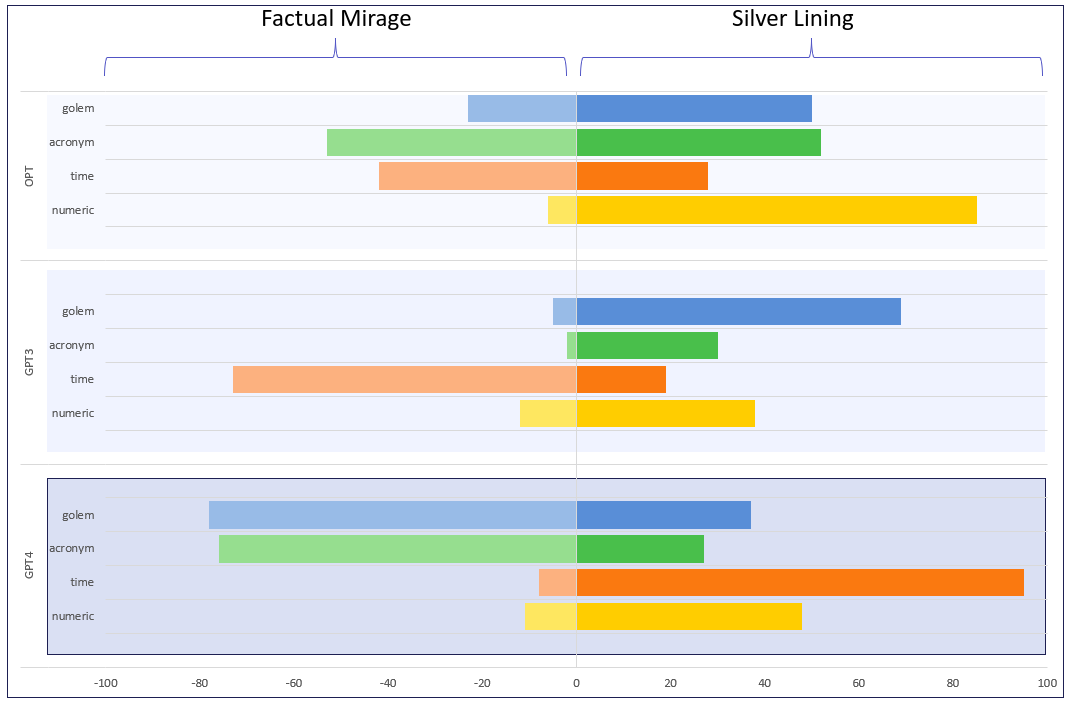
\includegraphics[width=\textwidth,height=9cm]{img/hvi.png}
    \caption{Hallucination Vulnerability Index \emph{(HVI)} for different hallucination categories for various LLMs \textcolor{red}{why does this figure have an arxiv link?}}
    \label{fig:hvi}
\end{figure}
% \qquad
% %\begin{table}[!ht]
%\tiny
%\centering
%\resizebox{0.32\textheight}{!}{%
\resizebox{0.9\columnwidth}{!}{%
\begin{tabular}{lll}
\toprule
\textbf{LLM} & \textbf{Size} & \textbf{HVI (0-100)}
\\ \midrule
\textbf{GPT-3}    &  175B       &   90 - 
\begin{tikzpicture}
\centering
\draw[red, very thick, fill=red] (0,0)  rectangle (5.62,.1);
\end{tikzpicture}
\\
\textbf{StableLM}    &  7B   &     82 - 
\begin{tikzpicture}
\centering
\draw[red, very thick, fill=red] (0,0)  rectangle (5.12,.1);
\end{tikzpicture}
\\
\textbf{GPT-2}    &   1.5B      &     70 - 
\begin{tikzpicture}
\centering
\draw[red, very thick, fill=red] (0,0)  rectangle (4.38,.1);
\end{tikzpicture}
\\
\textbf{Vicuna}     & 13B      &   62 - 
\begin{tikzpicture}
\centering
\draw[orange, very thick, fill=orange] (0,0)  rectangle (3.88,.1);
\end{tikzpicture}  
\\
\textbf{MPT}    &  7B    &     59 - 
\begin{tikzpicture}
\centering
\draw[orange, very thick, fill=orange] (0,0)  rectangle (3.69,.1);
\end{tikzpicture}   
\\
\textbf{LLaMA}    &  65B    &     57 - 
\begin{tikzpicture}
\centering
\draw[orange, very thick, fill=orange] (0,0)  rectangle (3.56,.1);
\end{tikzpicture}   
\\
\textbf{GPT-3.5}   &    175B      &     53 - 
\begin{tikzpicture}
\centering
\draw[orange, very thick, fill=orange] (0,0)  rectangle (3.31,.1);
\end{tikzpicture}
\\
\textbf{Dolly}    &   12B    &    49 - 
\begin{tikzpicture}
\centering
\draw[violet, very thick, fill=violet] (0,0)  rectangle (3.06,.1);
\end{tikzpicture} 
\\
\textbf{OPT}    &   175B   &     48 - \begin{tikzpicture}
\centering
\draw[violet, very thick, fill=violet] (0,0)  rectangle (3,.1);
\end{tikzpicture}   
\\
\textbf{GPT-4}    &   1.7T    &      47 - \begin{tikzpicture}
\centering
\draw[violet, very thick, fill=violet] (0,0)  rectangle (2.94,.1);
\end{tikzpicture}  
\\
\textbf{Alpaca}   &   65B    &     40 - \begin{tikzpicture}
\centering
\draw[violet, very thick, fill=violet] (0,0)  rectangle (2.5,.1);
\end{tikzpicture}   
\\
\textbf{BLOOM}   &   176B     &   38 - \begin{tikzpicture}
\centering
\draw[blue, very thick, fill=blue] (0,0)  rectangle (2.38,.1);
\end{tikzpicture}  
\\
\textbf{T0}    &      11B    &     36 - \begin{tikzpicture}
\centering
\draw[blue, very thick, fill=blue] (0,0)  rectangle (2.25,.1);
\end{tikzpicture}  
\\
\textbf{XLNet}   &   340M     &      36 - \begin{tikzpicture}
\centering
\draw[blue, very thick, fill=blue] (0,0)  rectangle (2.25,.1);
\end{tikzpicture}  
\\
\textbf{T5}    &    11B      &     32 - \begin{tikzpicture}
\centering
\draw[blue, very thick, fill=blue] (0,0)  rectangle (2.0,.1);
\end{tikzpicture}  
\\
% ERNIE           &     40 - \begin{tikzpicture}
% \centering
% \draw[violet, very thick, fill=violet] (0,0)  rectangle (2,.5);
% \end{tikzpicture}  
% \\
% ALBERT          &   33 - \begin{tikzpicture}
% \centering
% \draw[blue, very thick, fill=blue] (0,0)  rectangle (1.8,.5);
% \end{tikzpicture}    
% \\
% DeBERTa         &     32 - \begin{tikzpicture}
% \centering
% \draw[blue, very thick, fill=blue] (0,0)  rectangle (1.6,.5);
% \end{tikzpicture}    
% \\
% ELECTRA         &    32 - \begin{tikzpicture}
% \centering
% \draw[blue, very thick, fill=blue] (0,0)  rectangle (1.8,.5);
% \end{tikzpicture}     
% \\
% RoBERTa         &    28 - \begin{tikzpicture}
% \centering
% \draw[blue, very thick, fill=blue] (0,0)  rectangle (1.4,.5);
% \end{tikzpicture}     
% \\
% BERT            &    26 - \begin{tikzpicture}
% \centering
% \draw[blue, very thick, fill=blue] (0,0)  rectangle (1,.5);
% \end{tikzpicture}     
% \ \ 
\bottomrule
\end{tabular}%
}
%%
%}


%\caption{A ranked list of LLMs based on HVI.}
%\label{tab:LLMs}
%\end{table}
%\vspace{-3mm}









\begin{comment}
%\begin{table}[!ht]
%\tiny
%\centering
\resizebox{\columnwidth}{!}{%
\begin{tabular}{lll}
\toprule
\textbf{LLM} & \textbf{Size} & \textbf{HVI (0-100)}
\\ \midrule
\textbf{GPT 4}    &  N/A       &   90 - \begin{tikzpicture}
\centering
\draw[red, very thick, fill=red] (0,0)  rectangle (5,.1);
\end{tikzpicture}
\\
\textbf{GPT 3.5}    &  1.3B   &     82 - \begin{tikzpicture}
\centering
\draw[red, very thick, fill=red] (0,0)  rectangle (4.6,.1);
\end{tikzpicture}
\\
\textbf{GPT 3}     & 175B      &   70 - \begin{tikzpicture}
\centering
\draw[red, very thick, fill=red] (0,0)  rectangle (4.4,.1);
\end{tikzpicture}  
\\
\textbf{GPT 2}    &   1.5B    &      47 - \begin{tikzpicture}
\centering
\draw[red, very thick, fill=red] (0,0)  rectangle (4.2,.1);
\end{tikzpicture}  
\\
\textbf{MPT}   &    7B      &     59 - \begin{tikzpicture}
\centering
\draw[orange, very thick, fill=orange] (0,0)  rectangle (4.0,.1);
\end{tikzpicture}
\\
\textbf{OPT}    &   125M      &     59 - \begin{tikzpicture}
\centering
\draw[orange, very thick, fill=orange] (0,0)  rectangle (3.8,.1);
\end{tikzpicture}
\\
\textbf{LLaMA}    &   7B    &    52 - \begin{tikzpicture}
\centering
\draw[orange, very thick, fill=orange] (0,0)  rectangle (3.5,.1);
\end{tikzpicture} 
\\
\textbf{BLOOM}   &   175B     &   49 - \begin{tikzpicture}
\centering
\draw[orange, very thick, fill=orange] (0,0)  rectangle (3.3,.1);
\end{tikzpicture}  
\\
\textbf{Alpaca}    &   7B   &     44 - \begin{tikzpicture}
\centering
\draw[orange, very thick, fill=orange] (0,0)  rectangle (3.1,.1);
\end{tikzpicture}   
\\
\textbf{Vicuna}    &  7B    &     44 - \begin{tikzpicture}
\centering
\draw[violet, very thick, fill=violet] (0,0)  rectangle (2.9,.1);
\end{tikzpicture}   
\\
\textbf{Dolly}   &   12B    &     44 - \begin{tikzpicture}
\centering
\draw[violet, very thick, fill=violet] (0,0)  rectangle (2.7,.1);
\end{tikzpicture}   
\\
\textbf{StableLM}    &  3B    &     44 - \begin{tikzpicture}
\centering
\draw[violet, very thick, fill=violet] (0,0)  rectangle (2.5,.1);
\end{tikzpicture}   
\\
\textbf{XLNet}   &   110M     &      42 - \begin{tikzpicture}
\centering
\draw[blue, very thick, fill=blue] (0,0)  rectangle (2.3,.1);
\end{tikzpicture}  
\\
\textbf{T0}    &      11B    &     42 - \begin{tikzpicture}
\centering
\draw[blue, very thick, fill=blue] (0,0)  rectangle (2.2,.1);
\end{tikzpicture}  
\\
\textbf{T5}    &    3B      &     41 - \begin{tikzpicture}
\centering
\draw[blue, very thick, fill=blue] (0,0)  rectangle (2.0,.1);
\end{tikzpicture}  
\\
% ERNIE           &     40 - \begin{tikzpicture}
% \centering
% \draw[violet, very thick, fill=violet] (0,0)  rectangle (2,.5);
% \end{tikzpicture}  
% \\
% ALBERT          &   33 - \begin{tikzpicture}
% \centering
% \draw[blue, very thick, fill=blue] (0,0)  rectangle (1.8,.5);
% \end{tikzpicture}    
% \\
% DeBERTa         &     32 - \begin{tikzpicture}
% \centering
% \draw[blue, very thick, fill=blue] (0,0)  rectangle (1.6,.5);
% \end{tikzpicture}    
% \\
% ELECTRA         &    32 - \begin{tikzpicture}
% \centering
% \draw[blue, very thick, fill=blue] (0,0)  rectangle (1.8,.5);
% \end{tikzpicture}     
% \\
% RoBERTa         &    28 - \begin{tikzpicture}
% \centering
% \draw[blue, very thick, fill=blue] (0,0)  rectangle (1.4,.5);
% \end{tikzpicture}     
% \\
% BERT            &    26 - \begin{tikzpicture}
% \centering
% \draw[blue, very thick, fill=blue] (0,0)  rectangle (1,.5);
% \end{tikzpicture}     
% \\ 
\bottomrule
\end{tabular}%
}
%\caption{A ranked list of LLMs based on HVI.}
%\label{tab:LLMs}
%\end{table}
%\vspace{-3mm}
\end{comment}    
% \begin{tabular}[b]{cc}\hline
%   Table head & Table head \\ \hline
%   Some values & Some values \\
%   Some values & Some values \\
%   Some values & Some values \\
%   Some values & Some values \\
%   Some values & Some values \\
%   Some values & Some values \\ \hline
% \end{tabular}
% \captionlistentry[table]{A table beside a figure}
% \captionsetup{labelformat=andtable}
% \caption{A table beside a figure}
% \end{figure*}

% \begin{minipage}{0.35\linewidth}
% 		% \caption{Caption }
% 		\label{tab:le}
% 		\centering
%   %\begin{table}[!ht]
%\tiny
%\centering
%\resizebox{0.32\textheight}{!}{%
\resizebox{0.9\columnwidth}{!}{%
\begin{tabular}{lll}
\toprule
\textbf{LLM} & \textbf{Size} & \textbf{HVI (0-100)}
\\ \midrule
\textbf{GPT-3}    &  175B       &   90 - \begin{tikzpicture}
\centering
\draw[red, very thick, fill=red] (0,0)  rectangle (5.62,.1);
\end{tikzpicture}
\\
\textbf{StableLM}    &  7B   &     82 - \begin{tikzpicture}
\centering
\draw[red, very thick, fill=red] (0,0)  rectangle (5.12,.1);
\end{tikzpicture}
\\
\textbf{GPT-2}    &   1.5B      &     70 - \begin{tikzpicture}
\centering
\draw[red, very thick, fill=red] (0,0)  rectangle (4.38,.1);
\end{tikzpicture}
\\
\textbf{Vicuna}     & 13B      &   62 - \begin{tikzpicture}
\centering
\draw[orange, very thick, fill=orange] (0,0)  rectangle (3.88,.1);
\end{tikzpicture}  
\\
\textbf{MPT}    &  7B    &     59 - \begin{tikzpicture}
\centering
\draw[orange, very thick, fill=orange] (0,0)  rectangle (3.69,.1);
\end{tikzpicture}   
\\
\textbf{LLaMA}    &  65B    &     57 - \begin{tikzpicture}
\centering
\draw[orange, very thick, fill=orange] (0,0)  rectangle (3.56,.1);
\end{tikzpicture}   
\\
\textbf{GPT-3.5}   &    175B      &     53 - \begin{tikzpicture}
\centering
\draw[orange, very thick, fill=orange] (0,0)  rectangle (3.31,.1);
\end{tikzpicture}
\\
\textbf{Dolly}    &   12B    &    49 - \begin{tikzpicture}
\centering
\draw[violet, very thick, fill=violet] (0,0)  rectangle (3.06,.1);
\end{tikzpicture} 
\\
\textbf{OPT}    &   175B   &     48 - \begin{tikzpicture}
\centering
\draw[violet, very thick, fill=violet] (0,0)  rectangle (3,.1);
\end{tikzpicture}   
\\
\textbf{GPT-4}    &   1.7T    &      47 - \begin{tikzpicture}
\centering
\draw[violet, very thick, fill=violet] (0,0)  rectangle (2.94,.1);
\end{tikzpicture}  
\\
\textbf{Alpaca}   &   65B    &     40 - \begin{tikzpicture}
\centering
\draw[violet, very thick, fill=violet] (0,0)  rectangle (2.5,.1);
\end{tikzpicture}   
\\
\textbf{BLOOM}   &   176B     &   38 - \begin{tikzpicture}
\centering
\draw[blue, very thick, fill=blue] (0,0)  rectangle (2.38,.1);
\end{tikzpicture}  
\\
\textbf{T0}    &      11B    &     36 - \begin{tikzpicture}
\centering
\draw[blue, very thick, fill=blue] (0,0)  rectangle (2.25,.1);
\end{tikzpicture}  
\\
\textbf{XLNet}   &   340M     &      36 - \begin{tikzpicture}
\centering
\draw[blue, very thick, fill=blue] (0,0)  rectangle (2.25,.1);
\end{tikzpicture}  
\\
\textbf{T5}    &    11B      &     32 - \begin{tikzpicture}
\centering
\draw[blue, very thick, fill=blue] (0,0)  rectangle (2.0,.1);
\end{tikzpicture}  
\\
% ERNIE           &     40 - \begin{tikzpicture}
% \centering
% \draw[violet, very thick, fill=violet] (0,0)  rectangle (2,.5);
% \end{tikzpicture}  
% \\
% ALBERT          &   33 - \begin{tikzpicture}
% \centering
% \draw[blue, very thick, fill=blue] (0,0)  rectangle (1.8,.5);
% \end{tikzpicture}    
% \\
% DeBERTa         &     32 - \begin{tikzpicture}
% \centering
% \draw[blue, very thick, fill=blue] (0,0)  rectangle (1.6,.5);
% \end{tikzpicture}    
% \\
% ELECTRA         &    32 - \begin{tikzpicture}
% \centering
% \draw[blue, very thick, fill=blue] (0,0)  rectangle (1.8,.5);
% \end{tikzpicture}     
% \\
% RoBERTa         &    28 - \begin{tikzpicture}
% \centering
% \draw[blue, very thick, fill=blue] (0,0)  rectangle (1.4,.5);
% \end{tikzpicture}     
% \\
% BERT            &    26 - \begin{tikzpicture}
% \centering
% \draw[blue, very thick, fill=blue] (0,0)  rectangle (1,.5);
% \end{tikzpicture}     
% \ \ 
\bottomrule
\end{tabular}%
}
%%
%}


%\caption{A ranked list of LLMs based on HVI.}
%\label{tab:LLMs}
%\end{table}
%\vspace{-3mm}









\begin{comment}
%\begin{table}[!ht]
%\tiny
%\centering
\resizebox{\columnwidth}{!}{%
\begin{tabular}{lll}
\toprule
\textbf{LLM} & \textbf{Size} & \textbf{HVI (0-100)}
\\ \midrule
\textbf{GPT 4}    &  N/A       &   90 - \begin{tikzpicture}
\centering
\draw[red, very thick, fill=red] (0,0)  rectangle (5,.1);
\end{tikzpicture}
\\
\textbf{GPT 3.5}    &  1.3B   &     82 - \begin{tikzpicture}
\centering
\draw[red, very thick, fill=red] (0,0)  rectangle (4.6,.1);
\end{tikzpicture}
\\
\textbf{GPT 3}     & 175B      &   70 - \begin{tikzpicture}
\centering
\draw[red, very thick, fill=red] (0,0)  rectangle (4.4,.1);
\end{tikzpicture}  
\\
\textbf{GPT 2}    &   1.5B    &      47 - \begin{tikzpicture}
\centering
\draw[red, very thick, fill=red] (0,0)  rectangle (4.2,.1);
\end{tikzpicture}  
\\
\textbf{MPT}   &    7B      &     59 - \begin{tikzpicture}
\centering
\draw[orange, very thick, fill=orange] (0,0)  rectangle (4.0,.1);
\end{tikzpicture}
\\
\textbf{OPT}    &   125M      &     59 - \begin{tikzpicture}
\centering
\draw[orange, very thick, fill=orange] (0,0)  rectangle (3.8,.1);
\end{tikzpicture}
\\
\textbf{LLaMA}    &   7B    &    52 - \begin{tikzpicture}
\centering
\draw[orange, very thick, fill=orange] (0,0)  rectangle (3.5,.1);
\end{tikzpicture} 
\\
\textbf{BLOOM}   &   175B     &   49 - \begin{tikzpicture}
\centering
\draw[orange, very thick, fill=orange] (0,0)  rectangle (3.3,.1);
\end{tikzpicture}  
\\
\textbf{Alpaca}    &   7B   &     44 - \begin{tikzpicture}
\centering
\draw[orange, very thick, fill=orange] (0,0)  rectangle (3.1,.1);
\end{tikzpicture}   
\\
\textbf{Vicuna}    &  7B    &     44 - \begin{tikzpicture}
\centering
\draw[violet, very thick, fill=violet] (0,0)  rectangle (2.9,.1);
\end{tikzpicture}   
\\
\textbf{Dolly}   &   12B    &     44 - \begin{tikzpicture}
\centering
\draw[violet, very thick, fill=violet] (0,0)  rectangle (2.7,.1);
\end{tikzpicture}   
\\
\textbf{StableLM}    &  3B    &     44 - \begin{tikzpicture}
\centering
\draw[violet, very thick, fill=violet] (0,0)  rectangle (2.5,.1);
\end{tikzpicture}   
\\
\textbf{XLNet}   &   110M     &      42 - \begin{tikzpicture}
\centering
\draw[blue, very thick, fill=blue] (0,0)  rectangle (2.3,.1);
\end{tikzpicture}  
\\
\textbf{T0}    &      11B    &     42 - \begin{tikzpicture}
\centering
\draw[blue, very thick, fill=blue] (0,0)  rectangle (2.2,.1);
\end{tikzpicture}  
\\
\textbf{T5}    &    3B      &     41 - \begin{tikzpicture}
\centering
\draw[blue, very thick, fill=blue] (0,0)  rectangle (2.0,.1);
\end{tikzpicture}  
\\
% ERNIE           &     40 - \begin{tikzpicture}
% \centering
% \draw[violet, very thick, fill=violet] (0,0)  rectangle (2,.5);
% \end{tikzpicture}  
% \\
% ALBERT          &   33 - \begin{tikzpicture}
% \centering
% \draw[blue, very thick, fill=blue] (0,0)  rectangle (1.8,.5);
% \end{tikzpicture}    
% \\
% DeBERTa         &     32 - \begin{tikzpicture}
% \centering
% \draw[blue, very thick, fill=blue] (0,0)  rectangle (1.6,.5);
% \end{tikzpicture}    
% \\
% ELECTRA         &    32 - \begin{tikzpicture}
% \centering
% \draw[blue, very thick, fill=blue] (0,0)  rectangle (1.8,.5);
% \end{tikzpicture}     
% \\
% RoBERTa         &    28 - \begin{tikzpicture}
% \centering
% \draw[blue, very thick, fill=blue] (0,0)  rectangle (1.4,.5);
% \end{tikzpicture}     
% \\
% BERT            &    26 - \begin{tikzpicture}
% \centering
% \draw[blue, very thick, fill=blue] (0,0)  rectangle (1,.5);
% \end{tikzpicture}     
% \\ 
\bottomrule
\end{tabular}%
}
%\caption{A ranked list of LLMs based on HVI.}
%\label{tab:LLMs}
%\end{table}
%\vspace{-3mm}
\end{comment}    
% 		% \resizebox{\textwidth}{!}{%
% 		% \begin{tabular}[width=\linewidth]{@{}lll@{}}
%   %   \toprule
%   %   \textbf{Student} & \textbf{week} & \textbf{grade} \\ 
%   %   \midrule
%   %   Ada Lovelace & 2 & A \\
% 		% 	Linus Thorvalds & 8 & A \\
% 		% 	Bruce Willis & 12 & F \\
% 		% 	Richard Stallman & 10 & B \\
% 		% 	Grace Hopper & 12 & A \\
% 		% 	Alan Turing & 8 & C \\
% 		% 	Bill Gates & 6 & D \\
% 		% 	Steve Jobs & 4 & E \\
%   %   \bottomrule
%   %   \end{tabular}}
% 	\end{minipage}
%  % \hfill
% 	\begin{minipage}{0.6\linewidth}
% 		\centering
% 		% \captionof{figure}{Caption_2}
% 		\label{figu:re}
% 		\begin{figure}
% [!htbp]
    \centering
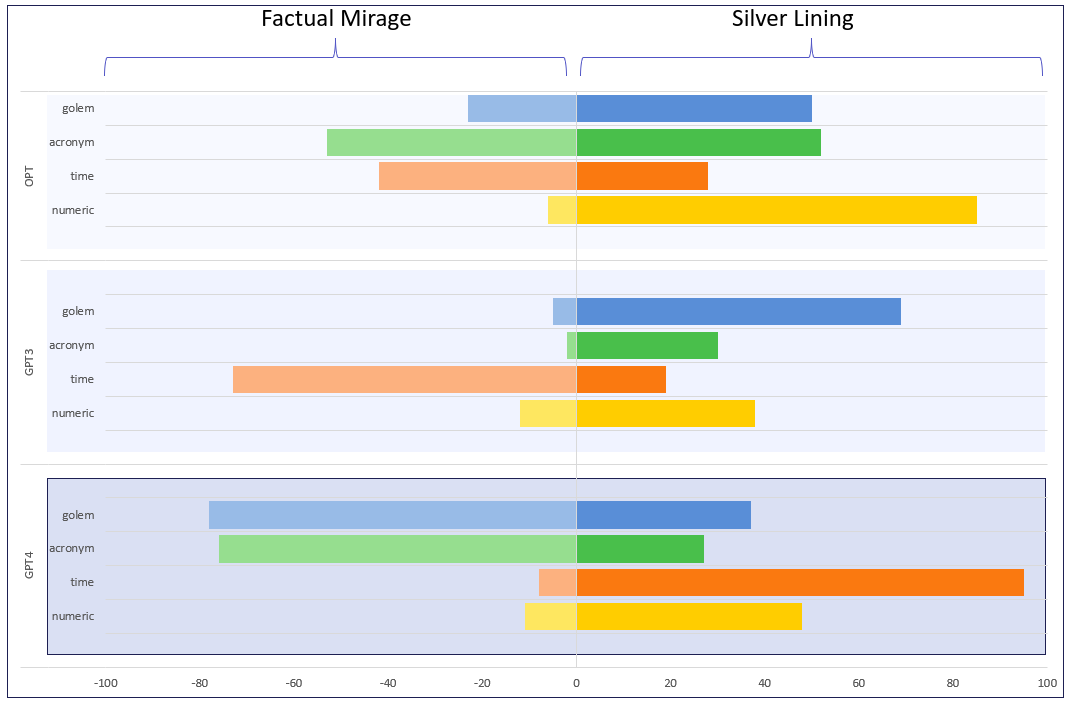
\includegraphics[width=\textwidth,height=9cm]{img/hvi.png}
    \caption{Hallucination Vulnerability Index \emph{(HVI)} for different hallucination categories for various LLMs \textcolor{red}{why does this figure have an arxiv link?}}
    \label{fig:hvi}
\end{figure}
%   % \includegraphics[width=0.8\textwidth]{Figs/Pair1.PNG}
% 	\end{minipage}

% \begin{table*}[!ht]%[H]
% \resizebox{0.98\textwidth}{!}{%
% \begin{tabular}{p{0.06\textwidth} | p{1.5\textwidth}} %{ll}
% \centering
% \toprule
% {\footnotesize \textbf{Prompt}} 
% & 
% \toprule
% \begin{footnotesize}
% \textit{USA's stance on Ukraine Russia war}
% \end{footnotesize}
% \\ \hline
% \rotatebox[origin=r]{90}{\parbox[c]{2cm}{\centering {\footnotesize \textbf{Hallucinated text}}}}
% & 
% \begin{footnotesize}
% {The official stance of the United States on the Russia-Ukraine war has been consistent in supporting Ukraine's sovereignty, territorial integrity, and the peaceful resolution of the conflict. The U.S. has condemned Russia's actions in annexing Crimea and its support for separatist movements in eastern Ukraine. Despite maintaining a diplomatic stance,  \colorbox{pink}{the U.S. President Barack Obama} stated that the United States would not deploy troops to Ukraine. Additionally, this lack of support extends to the withholding of financial and military assistance, including military equipment, training, and advisory support. This \colorbox{pink}{sentiment was reiterated} by \colorbox{pink}{Paul Altman} during a press review at the White House...}
% \end{footnotesize}
% \\ \hline
% \rotatebox[origin=r]{90}{\parbox[c]{2cm}{\centering {\footnotesize \textbf{Mitigated text\\\textcolor{blue}{ENTROPY\textsubscript{BB}}}}}}
% & 
% \begin{footnotesize}
% The official stance of the \colorbox{violet}{\textcolor{white}{government}} on the \colorbox{violet}{\textcolor{white}{ongoing}} war has been consistent in supporting \colorbox{violet}{\textcolor{white}{ resolution}} of the conflict. The \colorbox{violet}{\textcolor{white}{government}} has \colorbox{violet}{\textcolor{white}{condemned Russia}} in \colorbox{violet}{\textcolor{white}{country}} and its support for separatist movements in eastern \colorbox{violet}{\textcolor{white}{Ukraine}}. Despite maintaining a \colorbox{violet}{\textcolor{white}{neutral}} stance, the \colorbox{violet}{\textcolor{white}{government}} stated that the \colorbox{violet}{\textcolor{white}{country}} would not deploy troops to \colorbox{violet}{\textcolor{white}{unknown}}. Additionally, this lack of support extends to the withholding of financial and \colorbox{violet}{\textcolor{white}{resources}}, including \colorbox{violet}{\textcolor{white}{administrative}}, \colorbox{violet}{\textcolor{white}{technical}}, and \colorbox{violet}{\textcolor{white}{legal}}. This sentiment was \colorbox{violet}{\textcolor{white}{echoed}} by \colorbox{violet}{\textcolor{white}{minister}} during a press review at the \colorbox{violet}{\textcolor{white}{conference}}...
% \end{footnotesize}
% \\ \hline
% \rotatebox[origin=r]{90}{\parbox[c]{2.5cm}{\centering {\footnotesize \textbf{Edit Suggestions\\\textcolor{blue}{FACTUALITY\textsubscript{GB}}}}}}
% & 
% \begin{footnotesize}
% The official stance of the United States on the Russia-Ukraine war has been consistent in supporting Ukraine's sovereignty, territorial integrity, and the peaceful resolution of the conflict. The U.S. has condemned Russia's actions in annexing Crimea and its support for separatist movements in eastern Ukraine. \colorbox{red}{\textcolor{white}{Despite maintaining a diplomatic stance, the U.S. President Barack Obama stated that the United States would not deploy troops to Ukraine.}}\colorbox{orange}{\textcolor{white}{Additionally, this lack of support extends to t-}} \colorbox{orange}{\textcolor{white}{he withholding of financial and military assistance, including military equipment, training, and advisory support.}} \colorbox{red}{\textcolor{white}{This sentiment was reiterated by Paul Altman during a press review at th-}} \colorbox{red}{\textcolor{white}{e White House}}...
% \end{footnotesize}
% \\ \bottomrule
% \end{tabular}%
% }
% \caption{A hallucination example pre- and post-mitigation using an NYT tweet as a prompt. (Top) An output sample from an LLM that involves hallucinated components; (Bottom) A "mitigated" sample that shows a reduction in hallucination.}
% \label{tab:hallucination_ex}
% %\acil{I recommend replacing this example with an example that has a factual hallucination. Reviewers may argue that the impact of replacing the detected HE words is inconsequential -- it does not significantly change the perception of the story.}
% \end{table*}

%\acil{The above para seems like lit survey. In that case, I think we should massage this into a subsection of sec 1.}

%\subsection{Performance Analysis of ENTROPY\textsubscript{BB} and FACTUALITY\textsubscript{GB}}

%\cref{fig:awesome_image1} and \cref{fig:awesome_image2} \acb{offer a comparative analysis of the proposed approaches}. \ac{Which figures are being referred here?}


%the following mitigation strategies: (i) we discuss the approach of automatically replacing high entropy words and phrases as a means to counteract hallucination; (ii) we delve into the method of highlighting specific sections of generated text and prompting the user to edit them, thereby presenting a human-in-the-loop solution.